\documentclass[ 10pt]{report}
\usepackage[a4paper, total={6.5in, 10in}]{geometry}
\usepackage{hyperref}
\usepackage{blindtext}
\usepackage{titlesec}
\usepackage{indentfirst}
\usepackage{graphicx}
\usepackage{xcolor}
\usepackage{array}
\usepackage{tikz}
\usepackage{pdfpages}

\graphicspath{ {./images/} }
\titleformat{\chapter}[hang]{\Huge\bfseries}{\thechapter}{0.5em}{}
\definecolor{ao(english)}{rgb}{0.0, 0.5, 0.0}
\setcounter{section}{1}
\def\checkmark{\tikz\fill[scale=0.4](0,.35) -- (.25,0) -- (1,.7) -- (.25,.15) -- cycle;} 

\hypersetup{
    colorlinks=true,
    linkcolor=black,   
    urlcolor=cyan,
}

\begin{document}
    \begin{titlepage}
        % Title Page
        \noindent\rule{\textwidth}{5pt} \\
        \begin{flushright}
            \Huge\textbf{A7 - System documentation} \\[2\baselineskip]
            \large\textbf{for} \\
            \huge\textbf{Crowd Quizmaker} \\[2\baselineskip]
            \large\textbf{Version 1.1} \\[2\baselineskip]
            \large\textbf{Prepared by} \LARGE\textbf{0N3 N16H7 PR0J3C7} \\[0.5\baselineskip]
            \normalsize{
                Suwat Inkaew 610610521 \\
                Kritsanaphong Tepweerakul 630610714 \\
                Kitpisan Tanngan 630610716 \\
                Chayanon Pitak 630610724 \\
                Nadtaphong Jandaboot 630610743 \\
                Woranut Kitchakan 630610760
            } \\[2\baselineskip]
            \large{\href{https://github.com/ChayanonPitak/261361-Project/}{https://github.com/ChayanonPitak/261361-Project/}}
        \end{flushright}
        \pagebreak

        \LARGE\textbf{Revision History} \\[0.5\baselineskip]
        \normalsize{
            \begin{tabular}{| m{8em} | m{6em} | m{20em} | m{5em} |}
                \hline
                \textbf{Name} & \textbf{Date} & \textbf{Reason for changes} & \textbf{Version}\\ 
                \hline\hline
                Chayanon & 23 Mar 2023 & Complete of Sprint\#2 & 1.0 \\
                \hline
                Chayanon & 30 Mar 2023 & Add A4 \& A6 & 1.1 \\
                \hline
            \end{tabular}
        }

    \end{titlepage}

    \pagenumbering{alph}

     % Table of Contents
     \phantomsection
     \addcontentsline{toc}{chapter}{Table of Contents}
     \renewcommand*\contentsname{Table of Contents}
     \tableofcontents
     \pagebreak

    \pagenumbering{arabic}
    % A1 - Project proposal
    \chapter{A1 - Project proposal}
    \section{Team profile}
        \begin{itemize}
            \item \textbf{Chayanon Pitak} as Project Manager, System Analyst and Developer
            
                \textbf{Skills}
                \begin{itemize}
                    \item \textbf{Web application development} on JavaScipt, Typescript, React.js, Solid.js, PHP, TailwindCSS.
                    \item \textbf{Software development} on Java, C, C++.
                    \item \textbf{Game development} on Unity using C\#.
                \end{itemize}

                \textbf{Experience}
                \begin{itemize}
                    \item Mostly college projects and personal projects.
                \end{itemize}
            \item \textbf{Kritsanaphong Tepweerakul} as Developer and Business Analyst
                
                \textbf{Skills}
                \begin{itemize}
                    \item \textbf{Web application development} on JavaScipt, Typescript, React, TailwindCSS, PHP, Laravel.
                    \item \textbf{Software development} on C, C++, C\#, Java, Python.
                    \item \textbf{Game development} on Spring boot/React Web-based Game, Unity.
                \end{itemize}
                
                \textbf{Experience}
                \begin{itemize}
                    \item SFML 2D-RPG Game.
                    \item CARIN. (Strategy-Game Project)
                    \item Gogoboard Automatic Watering.
                    \item Store Website.
                \end{itemize}

                \item \textbf{Woranut Kitchakan} as Designer

                \textbf{Skills}
                \begin{itemize}
                    \item \textbf{Web application development} on JavaScipt, Typescript, React, TailwindCSS, Laravel.
                    \item \textbf{Software development} on C++, Java.
                    \item \textbf{Game development} on C++, Spring boot/React Web-based Game.
                \end{itemize}

                \textbf{Experience}
                \begin{itemize}
                    \item SFML Platform games.
                    \item CARIN. (Strategy-Game Project)
                    \item Gogoboard Automatic clothes drying machine.
                \end{itemize}

            \item \textbf{Kitpisan Tanngan} as Developer and Designer
                \textbf{Skills}
                \begin{itemize}
                    \item \textbf{Web application development} on JavaScipt, Typescript, React, TailwindCSS, Laravel.
                    \item \textbf{Software development} on  C++, Java.
                    \item \textbf{Game development} on C++, Java.
                \end{itemize}
            
                \textbf{Experience}
                \begin{itemize}
                    \item Turn-base Game Project.
                    \item Gogoboard Automatic roof for plants.
                \end{itemize}

            \item \textbf{Nadtaphong Jandaboot} as Tester and Designer
            
                \textbf{Skills}
                \begin{itemize}
                    \item \textbf{Web application development} on TailwindCSS.
                    \item \textbf{Software development} on C++.
                    \item \textbf{Art and Editing} on Photoshop. 
                \end{itemize}

                \textbf{Experience}
                \begin{itemize}
                    \item Mostly a art designer and sometimes front-end developer in projects. 
                \end{itemize}

            \item \textbf{Suwat Inkaew} as Tester
            \textbf{Skills}
                \begin{itemize}
                    \item \textbf{Web application development} on a little bit of JavaScipt, Typescript, React, TailwindCSS.
                    \item \textbf{Software development} on C, C++ and a little bit of C\#, Java.
                \end{itemize}
                
                \textbf{Experience}
                \begin{itemize}
                    \item SCRATCH Game.
                    \item CARIN(Tower Defense Game).
                    \item Review Website.
                    \item Card Game Project.
                \end{itemize}

        \end{itemize}

    \pagebreak
    \section{Crowd quizmaker}
    Students and lecturers generate quiz and answers. Quizzes can be edited, commented, voted and rated (e.g. quiz-maker)

    \section{Problem statement}
    
    Nowadays "Social network" is very popular for people to hang out on, they can see what their follower are doing, they can interact with follower and they can share their own content.

    But there is no "Examination Social Network" yet. Which can be a way to evaluate student's knowledge and let them to compete with each other that also fun for the student. For example, in the past Internet and Online Community course (261111) have a traditional examination, which is boring and not interactive. But if we have a "Examination Social Network" that can be a way to evaluate student's knowledge and let them to compete with each other that also fun for the student.
    
    \pagebreak
    \section{Solution}

    \subsection{Facebook group}
    \begin{center}
        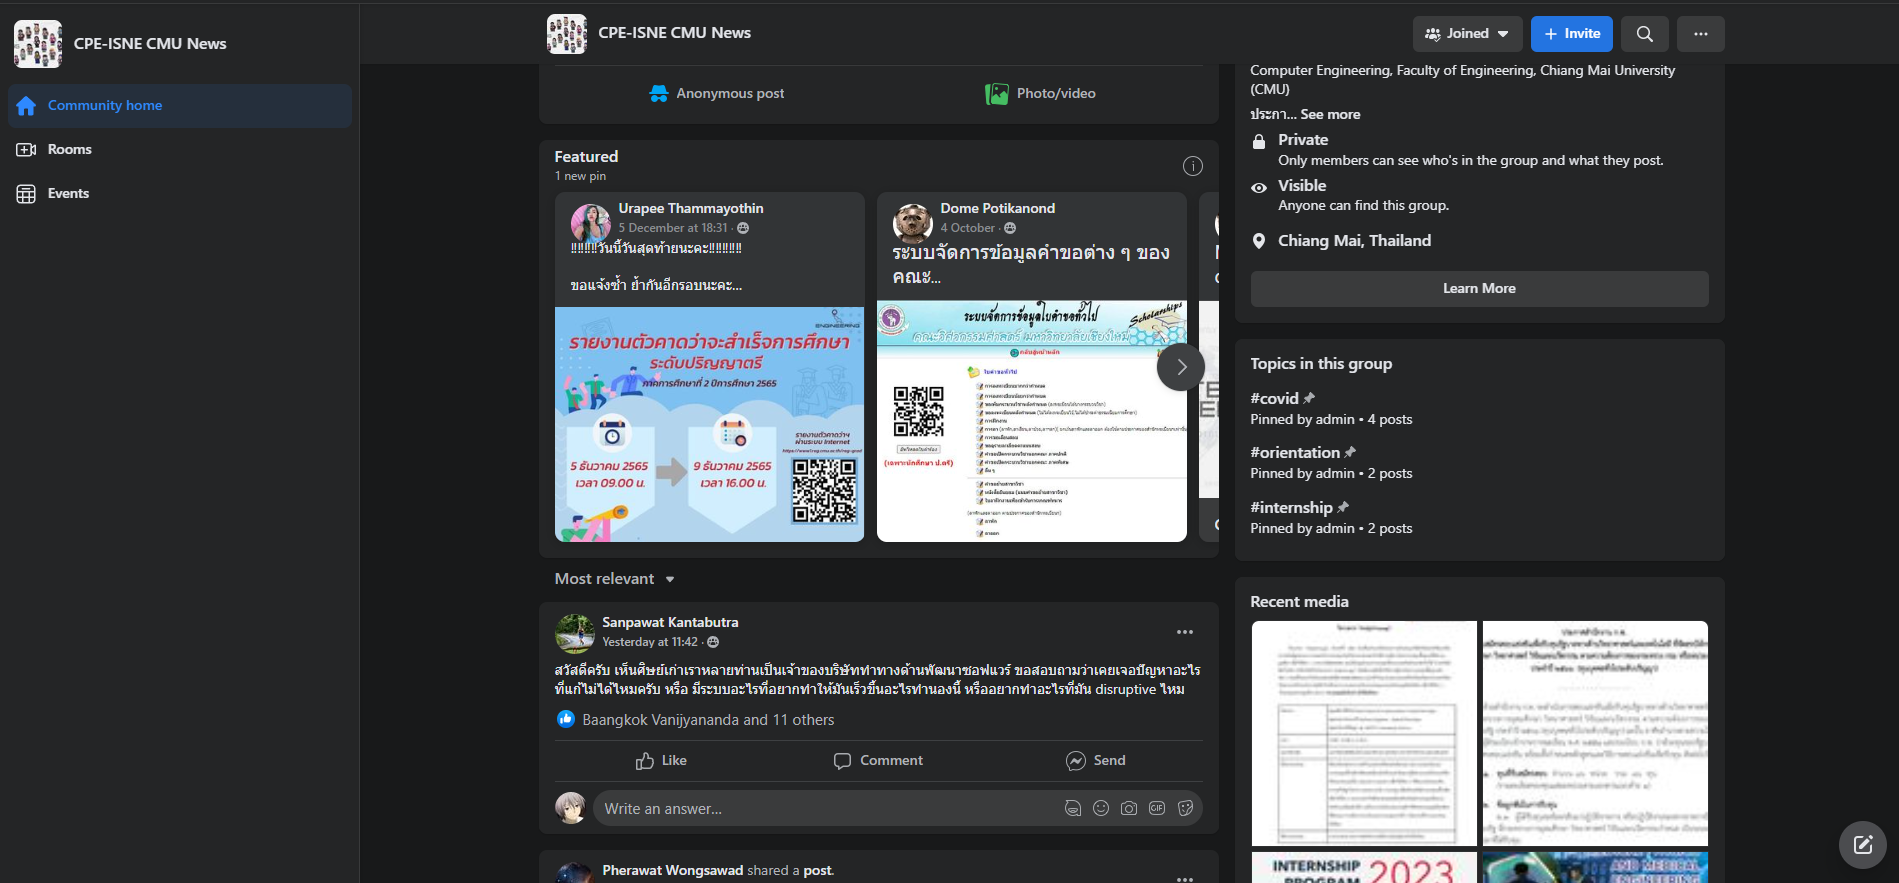
\includegraphics[height=150px]{facebook_group.png}
    \end{center}

    \textbf{Facebook group} is a group platform created by Meta. It let people with same interest to gather or lecturer can communicate with student. Also it is a way to let people create post (including quiz) and interact with each other. But it cannot evaluate student performance nor quiz quality and managing posts into topics/quizes is very hard or impossible to do.

    \subsection{Quiz-maker}
    \begin{center}
        
\includegraphics[height=150px]{quiz-maker.png}
    \end{center}
    
    \textbf{Quiz-maker} is a quiz creation platform. User can create quizzes of their own topic and share to others. It have great evaluation but lack of interaction and quizzes quality review from other users is impossible.
    
    
    \subsection{Kahoot!}
    \begin{center}
        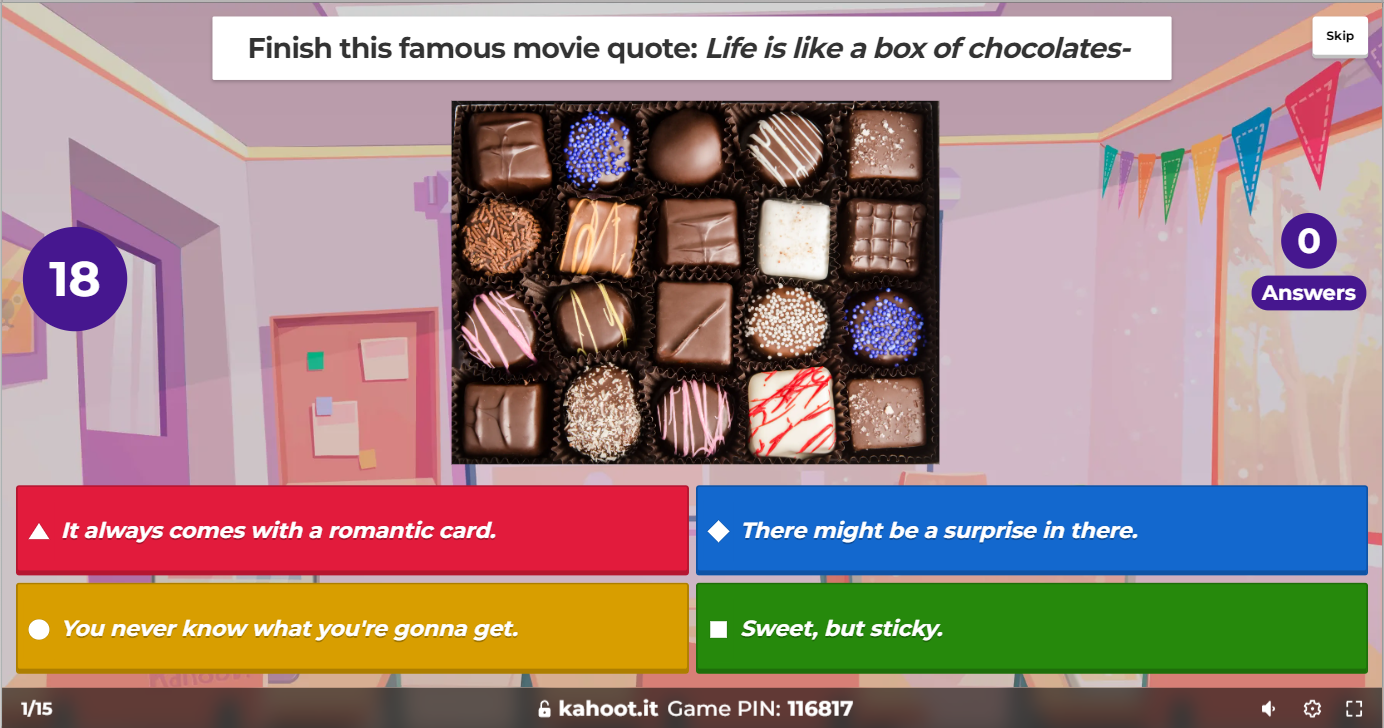
\includegraphics[height=150px]{kahoot.png}
    \end{center}
    
    \textbf{Kahoot} is a game-based learning platform. It let lecturer create questions according to topics and student can syncronously answer the questions with intensive environment. It have great evaluation and fun. But students cannot contribute their own quiz to existing quizzes.

    \subsection{Learning managament syatems (LMS) - Moodle, Blackboard, Canvas, etc.}
    \begin{center}
        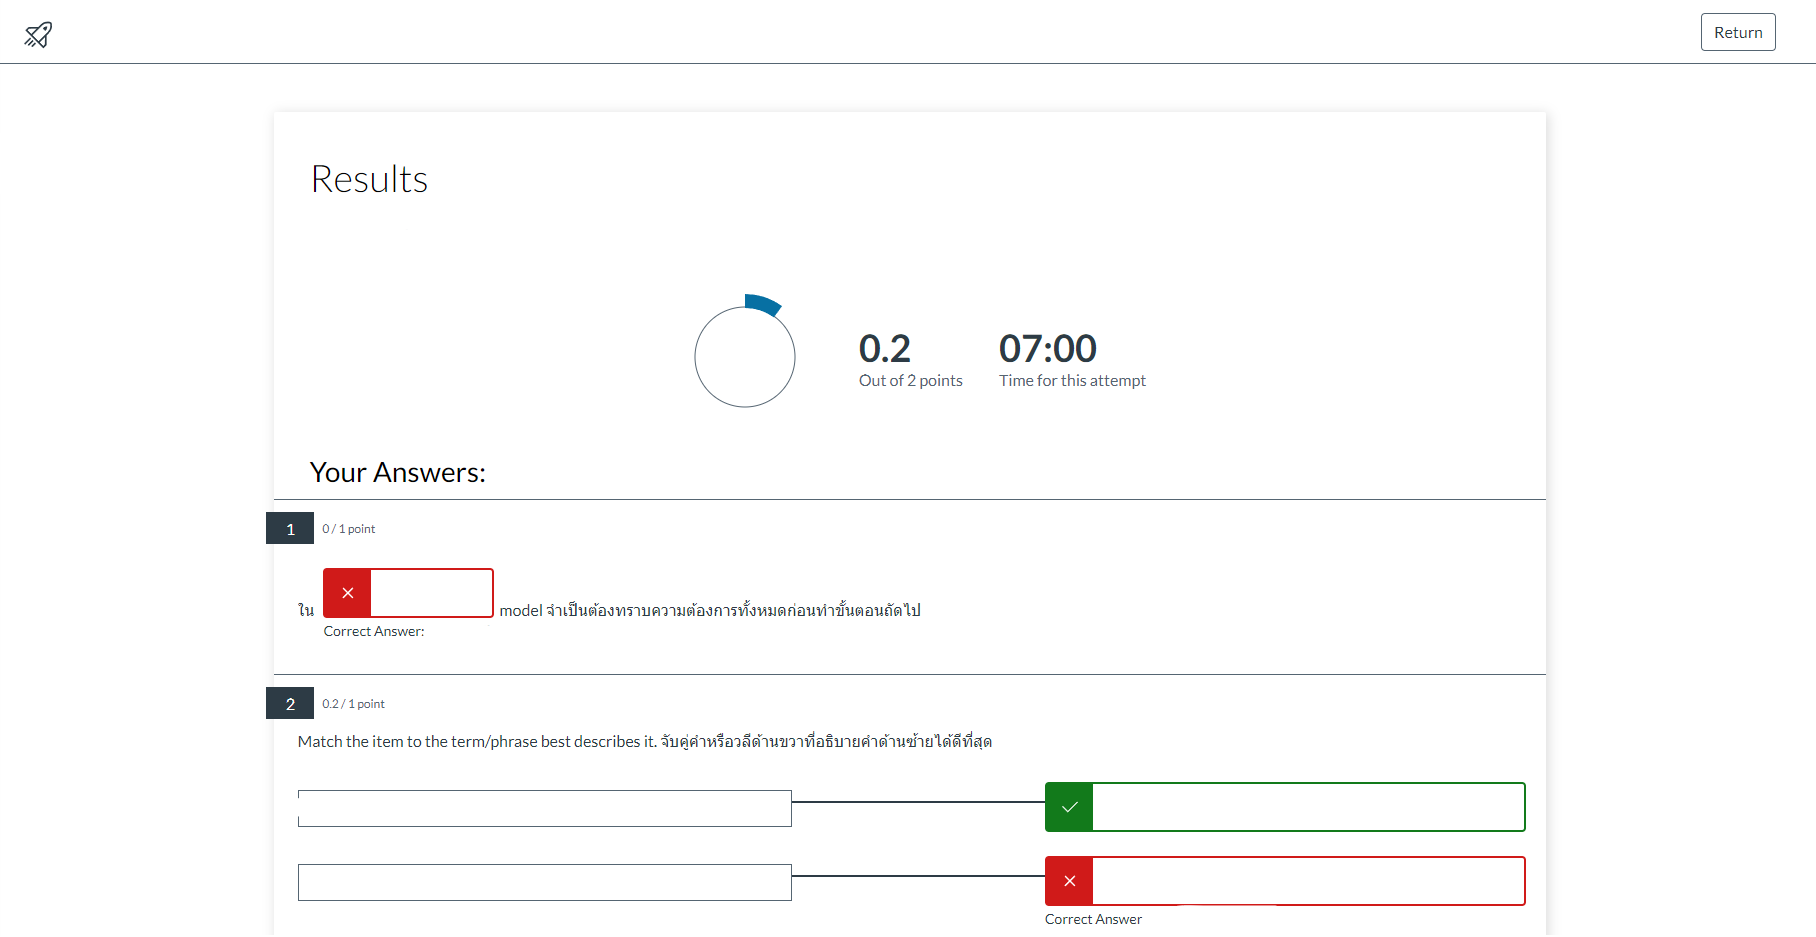
\includegraphics[height=150px]{LMS.png}
    \end{center}

    \textbf{Learning management system (LMS)} is an application that automates the administration, tracking, and reporting of training events.\footnote{Ryann K. Ellis, Field Guide to Learning Management Systems, Learning Circuits, 2009, p.1} It have great evaluation and grading, but quizzes looks like traditional examination.

    \pagebreak
    \section{Contribution}

    In general, quiz is created by one person or one group. It makes the number of quiz and variety of quiz is low. We have an inspiration of Facebook group which everyone in the groups can contribute to a topic, which will increase the variety and number of quiz. The process of creating quiz is as follows: define questions, define choices, define correct answers, have a system that can comment or vote on the quiz created by others to review the quality and correctness of the quiz, have a system that can evaluate the quality of the quiz.

    \subsection{Comparison to existing solutions}
    
    \begin{itemize}
        \item Facebook groups
        \begin{center}
            \begin{tabular}{| m{10em} | m{12em} | m{12em} |}
                \hline
                 & Facebook group & Our solution \\ 
                \hline\hline
                Quiz creation & Creating posts & \textcolor{ao(english)}{Creating quizzes with defined format} \\  
                \hline
                Quiz contribution & Everyone in group or group moderator approval & \textcolor{ao(english)}{Defined by subject creator} \\
                \hline
                Quiz validation & - & \textcolor{ao(english)}{Pre-defined format} \\
                \hline
                Quiz quality review & Reactions and Comments & \textcolor{ao(english)}{Pre-defined rubrics} \\
                \hline
                User evaluation & Manually & \textcolor{ao(english)}{User dashboard} \\
                \hline
            \end{tabular}
        \end{center}

        \item Quiz-maker
        \begin{center}
            \begin{tabular}{| m{10em} | m{12em} | m{12em} |}
                \hline
                 & Quiz-maker & Our solution \\ 
                \hline\hline
                Quiz creation & \textcolor{ao(english)}{Creating quizzes with defined format} & \textcolor{ao(english)}{Creating quizzes with defined format} \\  
                \hline
                Quiz contribution & Quiz creator & \textcolor{ao(english)}{Defined by subject creator} \\
                \hline
                Quiz validation & \textcolor{ao(english)}{Pre-defined format} & \textcolor{ao(english)}{Pre-defined format} \\
                \hline
                Quiz quality review & - & \textcolor{ao(english)}{Pre-defined rubrics} \\
                \hline
                User evaluation & \textcolor{ao(english)}{User dashboard} & \textcolor{ao(english)}{User dashboard} \\
                \hline
            \end{tabular}
        \end{center}

        \pagebreak
        \item Kahoot!
        \begin{center}
            \begin{tabular}{| m{10em} | m{12em} | m{12em} |}
                \hline
                 & Kahoot! & Our solution \\ 
                \hline\hline
                Quiz creation & \textcolor{ao(english)}{Creating quizzes with defined format} & \textcolor{ao(english)}{Creating quizzes with defined format} \\  
                \hline
                Quiz contribution & Quiz creator & \textcolor{ao(english)}{Defined by subject creator} \\
                \hline
                Quiz validation & \textcolor{ao(english)}{Pre-defined format} & \textcolor{ao(english)}{Pre-defined format} \\
                \hline
                Quiz quality review & Stars rating & \textcolor{ao(english)}{Pre-defined rubrics} \\
                \hline
                User evaluation & \textcolor{ao(english)}{User dashboard} & \textcolor{ao(english)}{User dashboard} \\
                \hline
                Syncronous activity & \textcolor{ao(english)}{\checkmark} & \textcolor{ao(english)}{\checkmark} \\
                \hline
            \end{tabular}
        \end{center}

        \item Learning management system
        \begin{center}
            \begin{tabular}{| m{10em} | m{12em} | m{12em} |}
                \hline
                 & LMS & Our solution \\ 
                \hline\hline
                Quiz creation & \textcolor{ao(english)}{Creating quizzes with defined format} & \textcolor{ao(english)}{Creating quizzes with defined format} \\  
                \hline
                Quiz contribution & Quiz creator  & \textcolor{ao(english)}{Defined by subject creator} \\
                \hline
                Quiz validation & \textcolor{ao(english)}{Pre-defined format} & \textcolor{ao(english)}{Pre-defined format} \\
                \hline
                Quiz quality review & - & \textcolor{ao(english)}{Pre-defined rubrics} \\
                \hline
                User evaluation & \textcolor{ao(english)}{User dashboard} & \textcolor{ao(english)}{User dashboard} \\
                \hline
            \end{tabular}
        \end{center}
    \end{itemize}

    \pagebreak
    \section{Stakeholder and User groups}
        \begin{itemize}
            \item \textbf{Product Owner}
            \begin{itemize}
                \item Professor Kampol Woradit as Internet and Online Community course lecturer. 
                \item Professor Sakgasit Ramingwong as Internet and Online Community course lecturer. 
            \end{itemize}
            \item \textbf{Study purpose}
            \begin{itemize}
                \item Lecturers
                \item Students
            \end{itemize}
            \item \textbf{Entertain purpose}
            \begin{itemize}
                \item Quiz Makers
                \item Who want to take advantage from their free time
                \item Who is interested in specific purpose
                \item Content creater who want to created content based on fan-quizzes
            \end{itemize}
        \end{itemize}
    

    \pagebreak
    \section{Technology feasibility study}
    We will create web application which is cross-platform friendly that can be use on mostly any device.

    \subsection{Tool and resources used}
    \begin{itemize}
        \item Figma for UI/UX design.
        \item Swagger for API design.
        \item diagrams.net for database design.
        \item HTML/CSS for web markdown and styling.
        \item Typescript for backend
        \item React.js for frontend framework.
        \item MySQL for database system.
        \item Prisma for database orm.
    \end{itemize}


    \pagebreak
    \section{Conclusion}

    We will create cross-playform web application that's looks like combination of Facebook groups and LMS, which lets user gather in groups and create quizzes together. Also users can review and rated quizzes quality.

    We will separete into two user groups.
    \begin{itemize}
        \item For \textbf{Lecturer and student}, lecturer can create and subject topic and let student create quizzes related to that topic. After that student will take each other quizzes to test their knowledge and rate their quizzes quality. This method make the quizzes become larger and more accurate for that subjects that student also have fun.
        \item For \textbf{Fans}, they can create quizezs related to their favorite topic and let others to contribute that topic.
    \end{itemize}

    % end A1

    % A2 - SRS
    \chapter{A2 - Software Requirement Specification}
    \section{Introduction}
        % Purpose
        \subsection{Purpose}
        Lecturer team of 261111 - Internet and Online Community, Chiang Mai University have created this course to create realize in technology, internet and online community and proper behaviour of using it. Originally, the course itself are using typical way of evaluate the understanding - assignments and exams which is one-way activities. The lecturer team have decided to create a new way of evaluate the understanding of the students by creating a quiz application that students also contribute the quiz creation from the knowledge they have learned from the course and try to answer and review the contributed quizzes. The application will be called Crowd Quizmaker.
        \subsection{Scope}
        Our software (Crowd Quizmaker) will be a cross-platform (Windows, MacOS, iOS, Android) web application that lecturer (or quiz admin) can create a quiz topic and students (or anyone - as quiz contributor) can contribute to a quiz - create, answer and review. Any users can be quizzes admin and/or quiz contributor and quizzes topic doesn't need to be academic purpose. Quizzes admin can specify what can quizzes contributor do.
        % Product Overview
        \subsection{Product Overview}
            % Product Perspective
            \subsubsection{Product Perspective}
            This product is a web application that can be accessed from any devices that have internet connection. The application will be a cross-platform (Windows, MacOS, iOS, Android) web application. The application is a quiz platform that any one can contribute to quizzes. The quizzes can be academic or non-academic.
            % Product Functions
            \subsubsection{Product Functions}
            The application consits of two part - Central system which provide the API, quizzes database storage and quizzes manager. And user client that allow any users to create quiz topic, manage quiz topic - moderate, manage, view and evaluate quiz content, contribute to quizzes - create, answer and review, and add support to Canvas LMS.
            % User Characteristics
            \subsubsection{User Characteristics}
            The user classes of this systems will be:
            \begin{enumerate}
                \item Administrator: Lecturer team of 261111 - Internet and Online Community, Chiang Mai University or any one who have the permission to manage the system. Responsible for manage, support and operate whole systems - both central system and clients.
                \item Course Lecturer: Any course lecturer who wish to use this system. Responsible for manage the quizzes topic, moderate quizzes content, evaluate quiz topic and/or Canvas LMS intregration.
                \item Course student: Student from courses. Responsible for Canvas LMS connection and contribute to quizzes from courses - create answer and review.  
                \item Quiz Admin: Anyone who want to create quizzes topic. Responsible for create/manage the quizzes topic, moderate quizzes content and evaluate quizz topic.
                \item Quiz Contributor: Anyone who want to contribute to quiz topic. Responsible for create, answer and review quizzes from quiz topics.
            \end{enumerate}
            % Limitations
            \subsubsection{Limitations}
            Currently we do not have any limitations from the requirements of stakeholders, but it may including but not limited to hardware performance limitstions, storage limitations, internet connection limitations, specific course content, local regulations and etc. We will update this subsection if we have any exact limitations to update.
        % Definitions
        \subsection{Definitions}
        \begin{itemize}
            \item \textbf{Central system or server}: The API provider, quizzes database storage and quizzes manager. Only accessible by administrator.
            \item \textbf{Client}: The user interface that allow any users to interact with our systems - Manage and moderate quiz topics and contribute to quizzes.
            \item \textbf{Quiz}: A set of questions and answers that can be answered by users.
            \item \textbf{Quiz Topic}: A topic that contain quizzes.
            \item \textbf{Quiz Admin}: An user that can create/manage quiz topic, moderate quizzes content and evaluate quiz topic.
            \item \textbf{Quiz Contributor}: An user that can contribute to quiz topic - create, answer and review quizzes.
            \item \textbf{Course lecturer or lecturer}: A course lecturer which have same permissions as Quiz Admin.
            \item \textbf{Course student or student}: A student which have same permissions as Quiz Contributor.
        \end{itemize}
    \pagebreak

    % References
    \section{References}
    \noindent ISO/IEC/IEEE 29148:2018 \\
    \href{https://ieeexplore.ieee.org/document/8559686}{https://ieeexplore.ieee.org/document/8559686} \\
    Systems and software engineering -- System and software requirements engineering -- System requirements specification \\\\

    \noindent CPE111 - Internet and Online Community facebook pages \\
    \href{https://www.facebook.com/CPE111/}{https://www.facebook.com/CPE111/} \\\\

    \noindent Canvas Learning Management System \\
    \href{https://www.instructure.com/en-au/canvas/}{https://www.instructure.com/en-au/canvas/} \\\\
    \pagebreak

    % Specific Requirements
    \section{Specific Requirements}
        % External Interfaces
        \subsection{External Interface}
            % System Interfaces
            \subsubsection{System Interfaces}
            The application will retrieve the registration information for the required course from "canvas.cmu.ac.th" in the form of JSON. This will provide the registration information for the application.
            \subsubsection{User Interfaces}
            The user interface will be simple to understand for all the user that uses this application. We will design a new user interface for our application using our experience and knowledge that doesn't consist of any standard. The reason is to eliminate the difficulty of the user's understanding of our application interface. 
            % Hardware Interfaces
            \subsubsection{Hardware Interfaces}
            No extra hardware interfaces are needed.
            % Software Interfaces
            \subsubsection{Software Interfaces}
            The application will use the GraphQL API from Canvas.
            % Communications Interfaces
            \subsubsection{Communications Interfaces}
            The application will use the HTTP protocol to communicate with the client. So, an internet connection is required.
        % Functions
        \subsection{Functions}
        The system shall
        \begin{enumerate}
            \item \textbf{Let user create quiz topic} which contains topic name, tags(optional), contributors(optional), format(multiple choices and/or text area), and distribution(question only, answer only or both).
            \item \textbf{Let quiz topic admin manage quiz topic} on topic name, contributors, format, and distribution and delete whole quiz topic.
            \item \textbf{Let quiz topic admin moderate quizzes content} on contributors' question, answer and review.
            \item \textbf{Let contrubutor create question to the quiz topic} based on quiz topic distribution and format. Contributor shall define the question, tag(depends on admin), answer(s) and correct answer(s).
            \item \textbf{Let contrubutor attempt to answer and review the question to the quiz topic} based on quiz topic distribution. System shall random the question based on distribution settings. User shall answer the question and review the question - rate, comment and/or report. (only quiz topic admin can see the review)
            \item \textbf{Evaluate the user's quiz attempt} which visualize the result of the quiz attempt. The result contains correct answer count on that attempt.
            \item \textbf{Let quiz topic admin evaluate the quiz topic} which visualize the result of the quiz attempt. The result contains correct answer count on questions and questions' review.
        \end{enumerate}
        % Usability Requirements
        \subsection{Usability Requirements}
        The system shall be able to operate normally without any errors or server issues. Also, it shall be simple to use for every user.
        % Performance Requirements
        \subsection{Performance Requirements}
        \begin{itemize}
        \item \textbf{Respond Time}: The system shall have a response time of fewer than 10 seconds for topic-related requests, except for adding contributors shall not have a responce time greater than 30 seconds.  
        \item \textbf{Throughput}: The system shall be able to handle 500 simultaneous users and shall be able to handle at least 100 requests per second.
        \item \textbf{Memory usage}: The system shall use no more than 1 GB of memory under normal conditions. 
        \item \textbf{CPU usage}: The system shall require atleast 4 core of CPU under normal conditions.
        \item \textbf{Storage}: The system shall be able to store up to atleast 1 TB of data.
        \item \textbf{Avalibility}: The system shall always be available to the user all the time.
        \end{itemize}
        % Logical Database Requirements
        \subsection{Logical Database Requirements}
        \begin{enumerate}
            \item The database shall be able to store user information and quiz data.
            \item The database shall always be able to provide data for the server most of the time.
            \item The database shall be able to ensure that each role of user can access their interface by their role.
        \end{enumerate}
        % Design Constraints
        \subsection{Design Constraints}
        \begin{itemize}
        \item \textbf{Time}: This application must be complete within 2-3 weeks.
        \item \textbf{Resource}: This application project team has 6 members.
        \item \textbf{Scalability}: The system must be design to support a minimum of 500 simultaneous users.
        \item \textbf{Deployment}: The system must be deployable to server-based and client-based infrastructure.
        \end{itemize}
        % Software System Attributes
        \subsection{Software System Attributes}
        \begin{itemize}
            \item \textbf{Reliability}: The system shall be able to perform an intended function without unexpected errors.
            \item \textbf{Maintainability}: The system shall be easy to maintain and update.
            \item \textbf{Portability}: The system shall be able to run on multiple operating system, including Window, Mac, Android and iOS.
        \end{itemize}
        % Supporting Information
        \subsection{Supporting Information}
        \begin{enumerate}
            \item The application shall be able to run on every modern browsers.
            \item The application shall not send any personal data of the user to the internet or an unknown source.
        \end{enumerate}
    \pagebreak

    % Verification
    \section{Verification}
        % External Interface
        \subsection{External Interface}
        % System Interfaces
        \subsubsection{System Interfaces}
            \begin{itemize}
                \item \textbf{Fetch from canvas}: After retrieving the course information, we will check the number of people on the course that are the same number people of information we have retrieved.
                \item \textbf{Import manually}: After imported manually, we will check that people are imported are really in this course.
            \end{itemize}
        % User Interfaces
        \subsubsection{User Interfaces}
            We will be using "User Acceptance Testing" in user interface by taking users to use the interface to check the simplest of the website.
        % Software Interfaces
        \subsubsection{Software Interfaces}
            We will test by checking whether the information is correct or not using "System Testing".
        % Communications Interfaces
        \subsubsection{Communications Interfaces}
            We won't test because HTTP protocal are standard system and already Verificate.
        % Function
        \subsection{Functions}
        We will be using "User Acceptance Testing" by finding the tester to test the function that is working properly or not.
        % Usability Requirements
        \subsection{Usability Requirements}
        Tester will test the app and send feedback about user experience.
        % Performance Requirements
        \subsection{Performance Requirements}
        \begin{itemize}
            \item \textbf{Respond Time}: Tester will test by reckon system's response time.  
            \item \textbf{Throughput}: Tester will test by sending requests to system.
            \item \textbf{Memory usage}: Tester will test by performance monitoring while running application.
            \item \textbf{CPU usage}: Tester will test by performance monitoring while running application.
            \item \textbf{Storage}: Tester will test by performance monitoring while running application.
            \item \textbf{Avalibility}: Tester will test by uptime monitoring.
            \end{itemize}
        % Logical Database Requirements
        \subsection{Logical Database Requirements}
        \begin{enumerate}
            \item Tester will test by send requests about user information and quiz data.
            \item Tester will test by uptime monitoring about data.
            \item Tester will test by access each rolls and test.
        \end{enumerate}
        % Design Constraints
        \subsection{Design Constraints}
        \begin{itemize}
            \item \textbf{Time}: Verification by scrum meeting, github Kanbanboard to check progress on implementation.
            \item \textbf{Resource}: Have a verification on skills and progress done by each members.
            \item \textbf{Scalability}: Verification by sending requests to system.
            \item \textbf{Deployment}: Verification by show connection between server and client.
        \end{itemize}
        % Software System Attributes
        \subsection{Software System Attributes}
        \begin{itemize}
            \item \textbf{Reliability}: Verification by test at most as possibe expected errors.
            \item \textbf{Maintainability}: Verification by change some part and it will done by few steps and don't have any causes to another parts.
            \item \textbf{Portability}: Verification by testing application on multiple operating system.
        \end{itemize}
        % Supporting Information
        \subsection{Supporting Information}
        \begin{enumerate}
            \item Verification by testing application on multiple modern browsers.
            \item Verification by penetration test.
        \end{enumerate}
    \pagebreak

    % end A2

    % A3 - Design Specification (A-DAPT)
    \chapter{A3 - Design Specification}
    Due to size issue, please visit \href{https://github.com/IkaWaAyuMu/261361-Project/blob/main/documents/A3/A3 1.0.pdf}{here} for the design specification.
    % end A3

    % A4 - Sprint #1
    \chapter{A4 - Sprint \#1}
    \pagebreak
    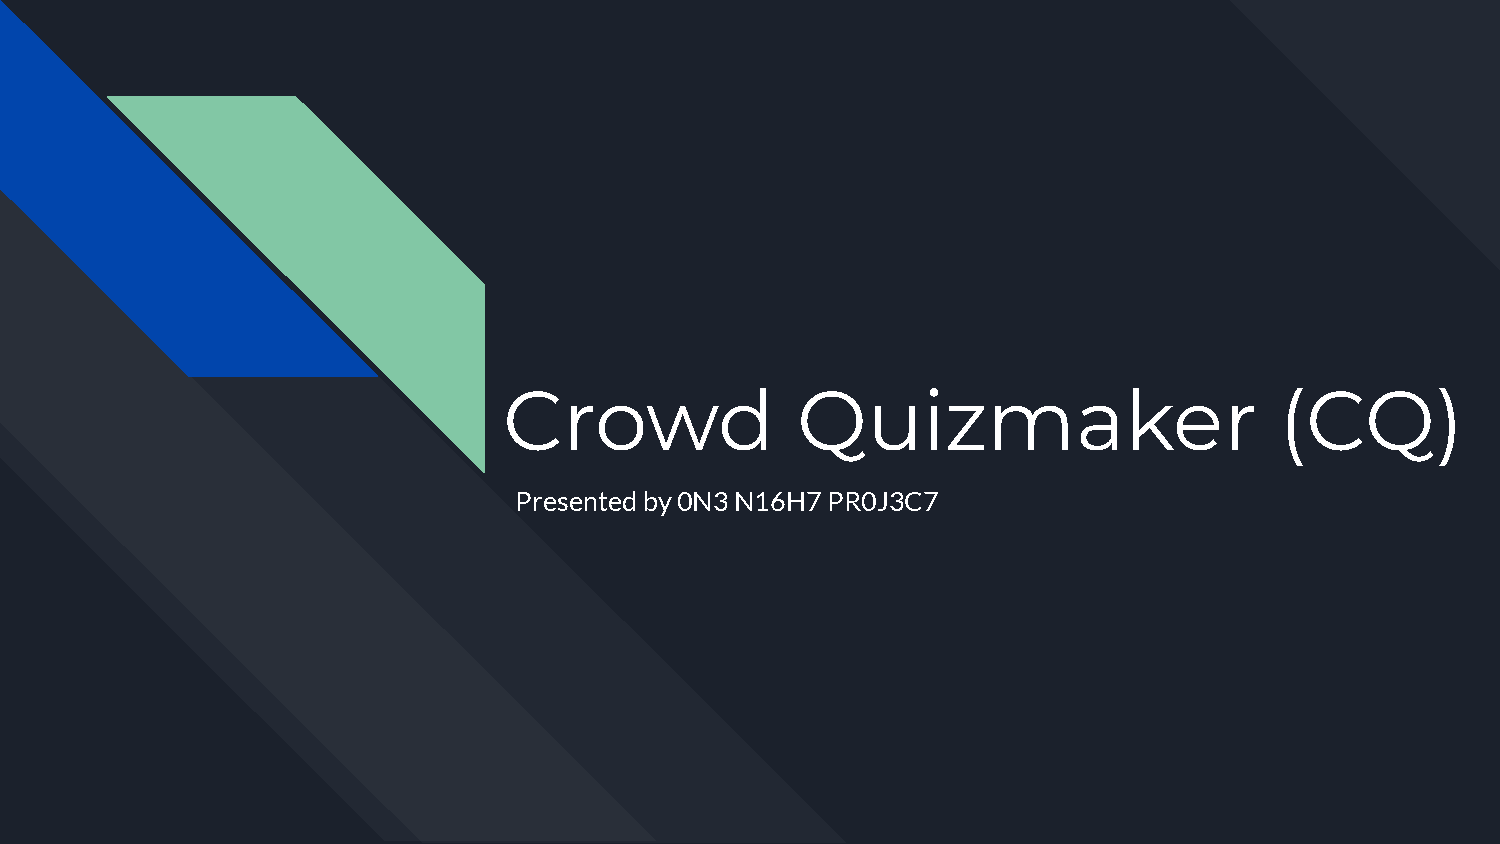
\includepdf[pages=-]{../A4/A4.pdf}

    % A5 - Test Document
    \chapter{A5 - Test Document}

    Software Name : Crowd Quizmaker
    Team name: 0N3 N16H7 PR0J3C7
    Tester names
    \begin{itemize}
        \item Suwat Inkaew 610610521
        \item Nadtaphong Jandaboot 630610743
    \end{itemize}
    \section{Scope}
        Our software (Crowd Quizmaker) will be a cross-platform (Windows, MacOS, iOS, Android) web application that lecturer (or quiz admin) can create a quiz topic and students (or anyone - as quiz contributor) can contribute to a quiz - create, answer and review. Any users can be quizzes admin and/or quiz contributor and quizzes topic doesn’t need to be academic purpose. Quizzes admin can specify what can quizzes contributor do.
    \section{Test scope}
    \begin{itemize}
        \item Item to be tested \begin{itemize}
            \item Desktop UI
            \item Sign up function
            \item Log in function
            \item Create Quiz Topic function
            \item Create Quiz (multiple choice format) function
            \item Setting allowance of Quiz function
            \item Manage Quiz function
            \item Delete Quiz function
            \item Attempt Quiz function
            \item Log out function
        \end{itemize}
        \item Item \textbf{NOT} to be tested \begin{itemize}
            \item Cross platform UI
            \item Review Quiz function
            \item Create Quiz (Subjective format) function
            \item Multiple correct choice function
            \item Quiz Info show function
        \end{itemize}
    \end{itemize}
    \section{Test exit criteria}
    \begin{itemize}
        \item Login and sign up authentication are working correctly
        \item UI and UX are satisfying the user
        \item Completing all specified types of testing with minimum number of errors, failures etc.
        \item Achieving a specified number of successful test cases
    \end{itemize}
    \section{Test overview}
    \begin{itemize}
        \item Unit Testing
        \item System Testing
        \item Integration Testing
        \item Acceptance Testing
    \end{itemize}
    \section{Test types}
    \begin{itemize}
        \item Unit Testing \begin{itemize}
                \item Test techniques : White Box Testing
                \item Description : Each unit tested by the developer to test thatunit working correctly.
                \item Tester : Developer
            \end{itemize}
        \item System Testing \begin{itemize}
                \item Test techniques : Black Box Testing
                \item Description : Done by the testing team by setting input randomly to check the return is according to requirement.
                \item Tester : Testing Team
            \end{itemize}
        \item Integration Testing \begin{itemize}
                \item Test techniques : Big-bang testing
                \item Description : Done by the testing team by runningapplications and trying all functions that integrate.
                \item Tester : Testing Team
            \end{itemize}
        \item Acceptance Testing \begin{itemize}
                \item Test techniques : Alpha Testing, Beta Testing
                \item Description : \begin{itemize}
                    \item Alpha testing is done by testing team by run a real-time scenario of quiz contributor and student
                    \item Beta testing done by TA
                \end{itemize}
                \item Tester : Testing Team, TA
            \end{itemize}
    \end{itemize}
    \section{Test result}
    \begin{itemize}
        \item Unit Testing \begin{itemize}
            \item Found some bugs and the developer already fixed it.
        \end{itemize}
        \item System Testing \begin{itemize}
            \item No holes detected, Already fix all holes.
        \end{itemize}
        \item Integration Testing \begin{itemize}
            \item All linked modules work normally.
        \end{itemize}
        \item Acceptance Testing \begin{itemize}
            \item Alpha test application works almost normally but still has some bugs in some functions.
            \item Beta test application working normally.
        \end{itemize}
    \end{itemize}
    \section{Recommendation}
    Base on the results of the testing effort, the following recommendation are provided
    \begin{itemize}
        \item Tester team should provide more testing techniques and more tests to verify the quality and reliability of the software.
        \item Tester team should provide more clear information to the developer team. This can be improved by providing more meetings or making a minor test document.
    \end{itemize}
    \section{Summary}
    The software testing effort for Crowd Quizmaker has been completed and the results are summarized in this report.
    
    The overall results of testing indicate that the software performs well. However, several defects were identified during testing, which have been documented and reported to the developer to fix the problem.
    
    The testing process was conducted using only manual testing techniques, including unit testing, system testing, integration testing and acceptance testing.
    
    The testing team encountered several challenges during the testing process, including lack of communication, diversity in the testing environment and inadequate testing, which affected the testing effort.
    
    Overall, the testing effort was successful in identifying defects and areas for improvement in the software.

    % A6 - Sprint #2
    \chapter{A6 - Sprint \#2}
    \pagebreak
    
\includepdf[pages=-]{../A6/A6.pdf}
    

    \pagenumbering{roman}
    % Appendix
    \chapter{Appendix}
        % Source code 
        \section{Source codes}
        Source code can be found at \href{https://github.com/ChayanonPitak/crowd-quizmaker/tree/main/source}{Github} (https://github.com/ChayanonPitak/crowd-quizmaker/tree/main/source)
        % Acronyms and Abbreviations
        \section{Acronyms and Abbreviations}
        \begin{itemize}
            \item \textbf{API}: Application Programming Interface
            \item \textbf{LMS}: Learning Management System
            \item \textbf{GB}: Gigabyte
            \item \textbf{HTTP}: Hypertext Transfer Protocol
            \item \textbf{TB}: Terabyte
        \end{itemize}

\end{document}